\documentclass[border=10pt]{standalone}

\usepackage{tikz}
\usepackage{tikzsymbols}
\usetikzlibrary{calc,patterns,shapes.geometric}

\def\centerarc[#1](#2)(#3:#4:#5){\draw[#1] ($(#2)+({#5*cos(#3)},{#5*sin(#3)})$) arc (#3:#4:#5);}

\begin{document}
	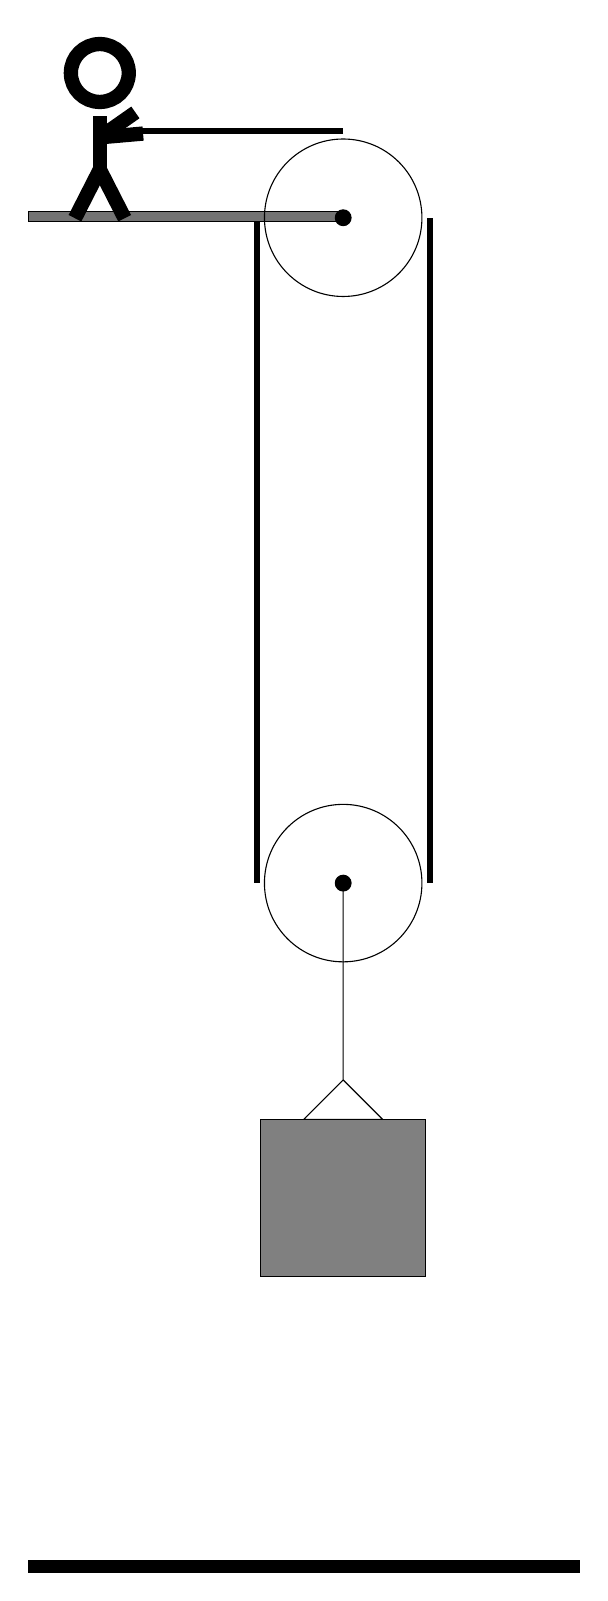
\begin{tikzpicture}
		%%%%% START %%%%%
		\draw[fill=black!55] (-2, 14) rectangle (2, 14.125);
		
		\draw (2, 5.6) circle (1);
		\draw[fill=black] (2, 5.6) circle (0.1);
		
		\draw (2, 14.05) circle (1);
		\draw[fill=black] (2, 14.05) circle (0.1);
		
		\draw (2, 5.6) -- (2, 3.1) -- (1.5, 2.6) -- (2.5, 2.6) -- (2, 3.1);
		\draw[fill=black!50] (0.95, 2.6) rectangle (3.05, 0.6);
		
		\draw[line width=0.75mm] (0.9, 14) -- (0.9, 5.6);
		\centerarc[line width=0.75mm](2, 5.6)(180:360:1.1);
		\draw[line width=0.75mm](3.1, 5.6) -- (3.1, 14.05);
		\centerarc[line width=0.75mm](2, 14.05)(0:90:1.1);
		\draw[line width=0.75mm](2, 15.15) -- (-1, 15.15);
		
		\node at (-1, 15.15) {\Strichmaxerl[10][-175][35]};
		
		\draw[fill=black] (-2, -3) rectangle (5, -3.15);
		%%%%% END %%%%%
	\end{tikzpicture}
\end{document}